To evaluate our solution we have performed experiments on a collection of 100 different proteins.
The average protein length is 78.12 amino acids spanning between 11 and 415.
The total running time of our fitting algorithm is around 2 minutes for the protein of length 415 on a 1.86GHz CPU.
There should be ample room for code optimizations as this has not been the focus of the project.

\section{Backbone fitting}
When fitting a protein to a given \Ca-trace we are interested in minimizing the RMSD while avoiding collisions.
In this section we will only consider the RMSD as the evaluation of our collision avoidance method  is delayed until Section \ref{sec:evaluation_handling_side-chains}. 

Typically, we are able to reach an RMSD less than 0.2 Å with our backbone fitting algorithm (Algorithm \ref{alg:ccd}).
This is considered satisfactory by the algorithms group at our department.
% We will wait until Sectionwill not consider the collision when evaluating the backbone fitting algorithm.
%In this experiment we have let our algorithm perform the same amount of work for different window sizes (ie. for small $w$ the number of window repetitions is large and vice versa).

As our fitting method performs CCD on a window within the backbone it is interesting to investigate the impact when varying the window size $w$.
Figure \ref{fig:rmsd_windowsize} shows the RMSD for four different window sizes $w$ as we repeat the fitting algorithm one to ten times.
After the first iteration we see that a small window size allows the fitting method to be flexible and reach a low RMSD quickly.
However, if $w$ is too small, the fitting does not improve as we repeat the algorithm.
This is because the chosen angles from a small window are too greedy and find local solutions that lead to an unfavorable global backbone conformation.
On the other hand if $w$ is too large, we see that the RMSD improves in each iteration but requires many iterations to reach a low RMSD.
The problem is caused by the end-effector becoming too large such that there is no clear direction towards the target since all the elements of the end-effector must go in different directions to reach their separate targets.
This results in small angular changes in each step of the CCD method and a slow RMSD convergence.
Thus, in determining the window size we must strike a balance between small and flexible to get fast convergence and large with the ability to better capture the optimal global solution.

\begin{figure}
	\centering
	\hspace*{-3.5mm}\includegraphics[width=1.1\columnwidth]{figures/plot_rmsd_convergence}
	\caption{woop}
	\label{fig:rmsd_convergence}
\end{figure}

	
%Figure \ref{fig:rmsd_convergence} shows the same tendency RMSD as a function of the window size $w$.
%%We see the same tendency as in Figure \ref{fig:rmsd_convergence}
%From the plot we see that the optimal window size is between 5 and 12 amino acids.
%For $w<5$ the RMSD increases.
%When $w>12$ the RMSD goes up because a large window makes it hard to converge towards the optimal set of angles.


\begin{figure}
	\centering
	\hspace*{-3.5mm}\includegraphics[width=1.1\columnwidth]{figures/plot_rmsd}
	\caption{RMSD as a function of the window size}
	\label{fig:rmsd_windowsize}
\end{figure}




\begin{figure}
	\centering
	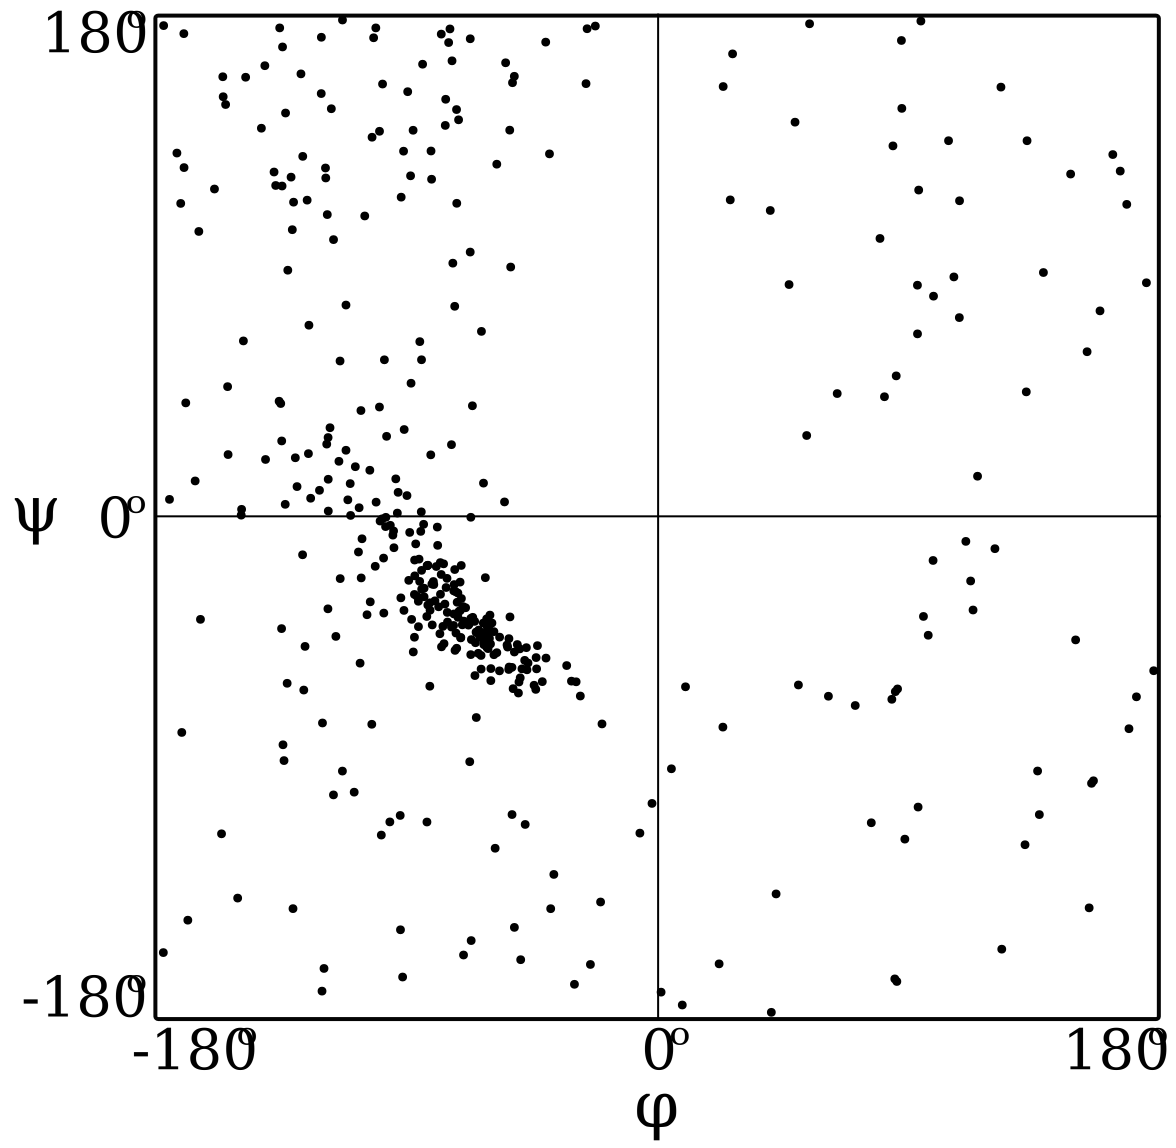
\includegraphics[width=0.85\columnwidth]{figures/plot_ramachandran}
	\caption{woop}
\end{figure}


\section{Side-chain handling}
\label{sec:evaluation_handling_side-chains}
\begin{figure}
	\centering
	\hspace*{-3.5mm}\includegraphics[width=1.1\columnwidth]{figures/plot_collisions}
	\caption{woop}
\end{figure}


%TODO billede af foldet backbone med \Ca trace
%TODO plot, x: antal kollisioner før fiksning, y: antal kollisioner efter fiksning


